\newpage
\vspace{6cm}
\section{METHODS}
\subsection{Use cases}
\hspace{0.7cm}To summarize the details of our application’s users and their interactions with the system, we created the following UML use case diagram:

\vspace{1.5cm}
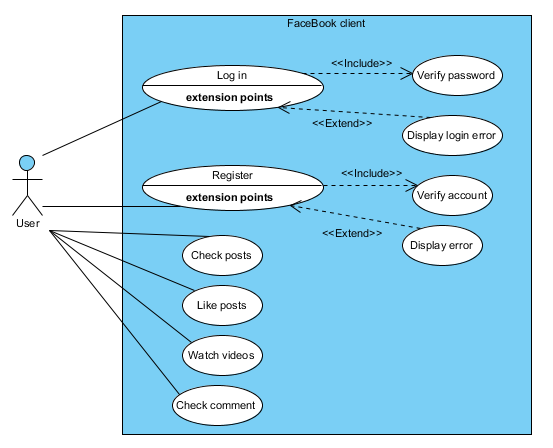
\includegraphics{Image/use_case.png}

\newpage
\subsection{Components}
\subsubsection{Activities}
\hspace{0.7cm}There are six main types of activities with different functions in our project:

\vspace{0.2cm} 1.	\textbf{Login/ Register activity}: provides people a way to create new accounts or access to the application if they already have ones.

\vspace{0.2cm}2.	\textbf{Main activity}: this is the default activity when users sign in. It is used to connect five main fragments: Homepage, Profile, Facebook Watch, Notifications and Menu.

\vspace{0.2cm}3.	\textbf{Zoom-in activities}: help users to watch full-screen videos and photos when needed.

\vspace{0.2cm}4.	\textbf{Notification detail activities}: support people to see further information of the notifications.

\vspace{0.2cm}5.	\textbf{Comment activities}: provide the user discussion about specific posts.

\vspace{0.2cm}6.	\textbf{Messenger activity}: stimulates the chatting section.

\subsubsection{Class diagram}
\hspace{0.5cm}Below is the UML class diagram of the application to provide further information about those activities’ classes, their attributes, operations, and the relationships among objects:

\vspace{1cm}
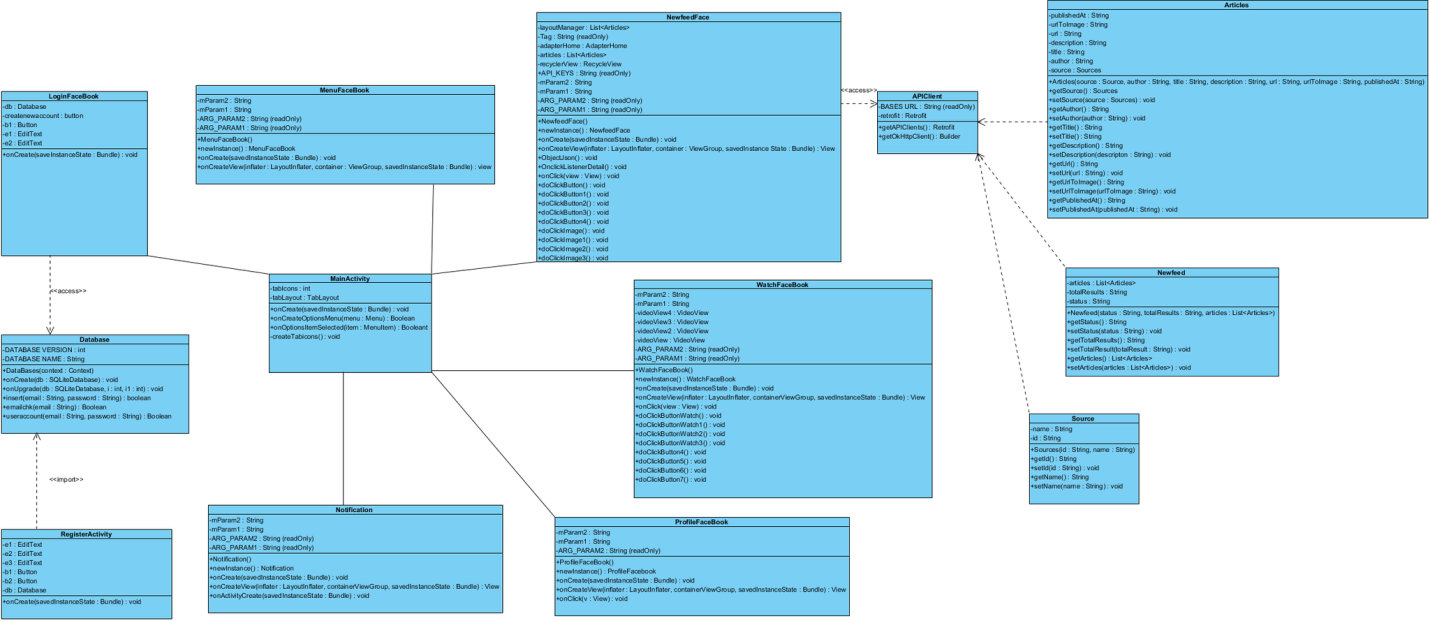
\includegraphics{Image/class_diagram.png}

\newpage
\subsection{Architecture}
\subsubsection{Layers}
\hspace{0.7cm}In order to achieve the use cases we listed above, our application must have two main layers:

\vspace{1cm}
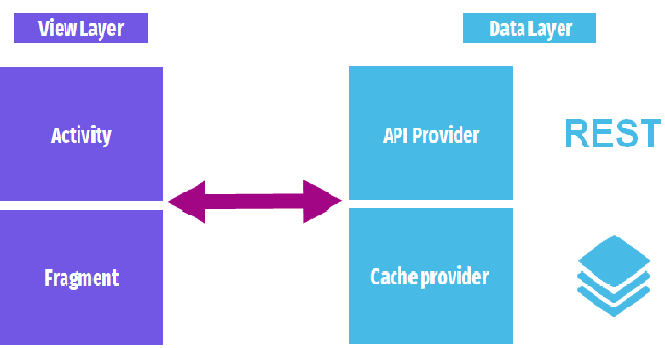
\includegraphics{Image/ArcLayer_new.png}

\begin{itemize}
  \item The first one is the VIEW LAYER which contains all the activities and fragments that users can see and interact with.
  \item The second one is the DATA LAYER. This layer is responsible for getting the data from remote data source using Representational State Transfer protocol and also from the database in the device cache.
\end{itemize}

\vspace{0cm}These two layers connect to each other through the request-respond relationship: users request data from the VIEW LAYER, then the DATA LAYER prepares and returns the needed information.
\subsubsection{Sequence diagram}
\hspace{0.5cm}To be more specific about how operations are carried out in our application, here is the system’s UML sequence diagram (Device is the VIEW LAYER; Account Database and Server are the DATA LAYER):


\newpage
\vspace{5cm}
\begin{center}
    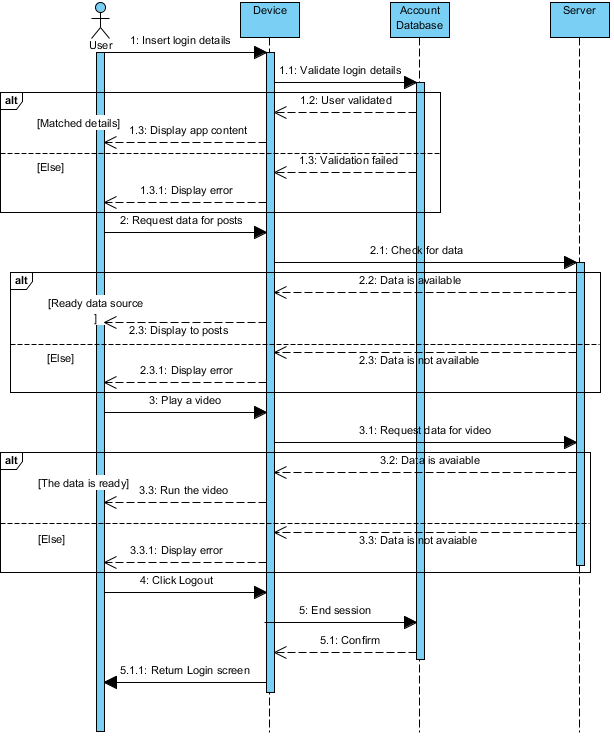
\includegraphics{Image/sequence_diagram.png}
    \\
    \caption{Figure 1: Case when the user already has an account}
\end{center}


\begin{center}
    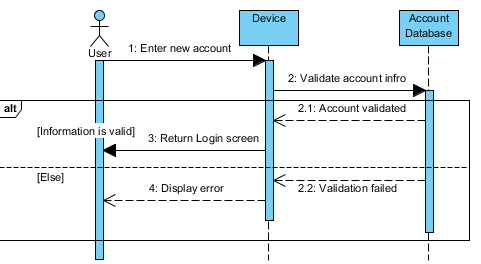
\includegraphics{Image/sequence_diagram_2.png}
    \\
    \caption{Figure 2: Case when the user registers a new account. Then login the same as Figure 1.}
\end{center}

\subsection{Networking}
\subsubsection{News feed}
\hspace{0.7cm}We created a post connected to “The US business news site” using openAPI with Representational State Transfer protocol (REST):

\vspace{0.5cm}\textbf{Step 1}: We made an API URL including three main parts to request data from the server:
\begin{itemize}
    \item \textbf{Domain}: “https://newsapi.org/v2”
    \item \textbf{Attribute}: to get data from the domain: “top-headlines”
    \item \textbf{API key}: to track and control how API is called: “23d4ed0e5fe84741ac530eb21b6ecc8a”
\end{itemize}
\hspace{0.7cm}Below is the need chunks of code to request and format API respectively:

\begin{minted}[mathescape, linenos]{java}
public static Retrofit retrofit;
public static final String BASES_URL="https://newsapi.org/v2/";
public static Retrofit getAPIClients() {
if (retrofit==null){
    retrofit=new Retrofit.Builder()
                .baseUrl(BASES_URL)
                .client(getOkHttpClient().build())
                .addConverterFactory(GsonConverterFactory.create()).build();
    }
return retrofit;
}
\end{minted}

\begin{minted}[mathescape, linenos]{java}
public interface APIKey {
    @GET("top-headlines")
        Call<Newfeed>getNewfeed(
    @Query("country") String country,
    @Query("apiKey") String apiKey);
}
\end{minted}

\vspace{0.5cm}\textbf{Step 2}: When the request is sent, the server will verify it and look for the appropriate resources to create the content returned accordingly.

\vspace{0.5cm}\textbf{Step 3}: When the verification is done, the server will return the result in JSON or XML format via HTTP or HTTPS.

\vspace{0.5cm}\textbf{Step 4}: Finally, when the application receives the data, it will display on the News feed screen. Below is the chunks of code to convert the status of an object into the byte string:
\begin{minted}[mathescape, linenos]{java}
@SerializedName("source")
@Expose
private  Sources source;
@SerializedName("author")
@Expose
private  String author;
@SerializedName("title")
@Expose
private  String title;
@SerializedName("description")
@Expose
private  String description;
@SerializedName("url")
@Expose
private  String url;
@SerializedName("urlToImage")
@Expose
private  String urlToImage;
@SerializedName("publishedAt")
@Expose
private  String publishedAt;
\end{minted}

\begin{minted}[mathescape, linenos]{java}
@SerializedName("status")
@Expose
private  String status;
@SerializedName("totalResults")
@Expose
private  String totalResults;
@SerializedName("articles")
@Expose
private List<Articles>articles;
\end{minted}

\begin{minted}[mathescape, linenos]{java}
@SerializedName("id")
@Expose
private String id;
@SerializedName("name")
@Expose
private String name;
\end{minted}

\vspace{0.5cm}In addition, we used a few libraries to support the API calling:
\begin{itemize}
    \item \underline{\textbf{Bumptech library}}: Glide supports fetching, decoding, and displaying video stills, images, and animated GIFs. Glide includes a flexible API that allows developers to plug in to almost any network stack.
    \item \underline{\textbf{Retrofit library}}: supports developers who convert APIs into Java Interfaces to easily connect to a REST service on the web.
    \item \underline{\textbf{Retrofit-gson library}}: a Java library used to convert Java objects into their JSON performances and vice versa.
    \item \underline{\textbf{PrettyTime library}}: used to normalize, calculate, and format time.
\end{itemize}

\subsubsection{Facebook watch}
\hspace{0.7cm}In this part, we used a stream server to upload videos. After that, we took the URL links from the server and called it back by using the embedded package. We also used "The Network Security Configuration" feature through an XML file in order to reach the needed links:

\begin{minted}[mathescape, linenos]{java}
<network-security-config>
    <base-config cleartextTrafficPermitted="true" />
</network-security-config>
\end{minted}





